\documentclass[aspectratio=169,professionalfonts]{beamer}

\usepackage{beamer-design-ff-aug}
\usepackage{setspace} % プリアンブルに追加
\setbeamercolor{structure}{fg=green!40!black}

\setbeamertemplate{navigation symbols}{}
\setbeamertemplate{footline}[frame number]

\title{Transformer入門 〜 ChatGPT の "T" を知る 〜}
\author{坪井 一馬}

% これはサンプルです
% 作成者のLT会での発表資料の作成過程に基づきます

\begin{document}

% \begin{frame}[plain]
%   \titlepage
% \end{frame}

{
  \usebackgroundtemplate{%
    
\includegraphics[
      width=\paperwidth,
      height=\paperheight
    ]{drawing.pdf}%
  }
  \setbeamertemplate{footline}{}

  \begin{frame}[plain]
  \end{frame}
}

\begin{frame}
  \frametitle{目次}
  \tableofcontents
\end{frame}

\section{自己紹介}

\begin{frame}{坪井 一馬 Kazuma TSUBOI}
    \centering
    % columns環境の開始（文字が上下中央に揃うようにオプション[c]を指定）
    \begin{columns}[c]
        \begin{column}{0.44\textwidth}
            \centering
            % [width=\textwidth] でカラム幅いっぱいに画像を拡大縮小
            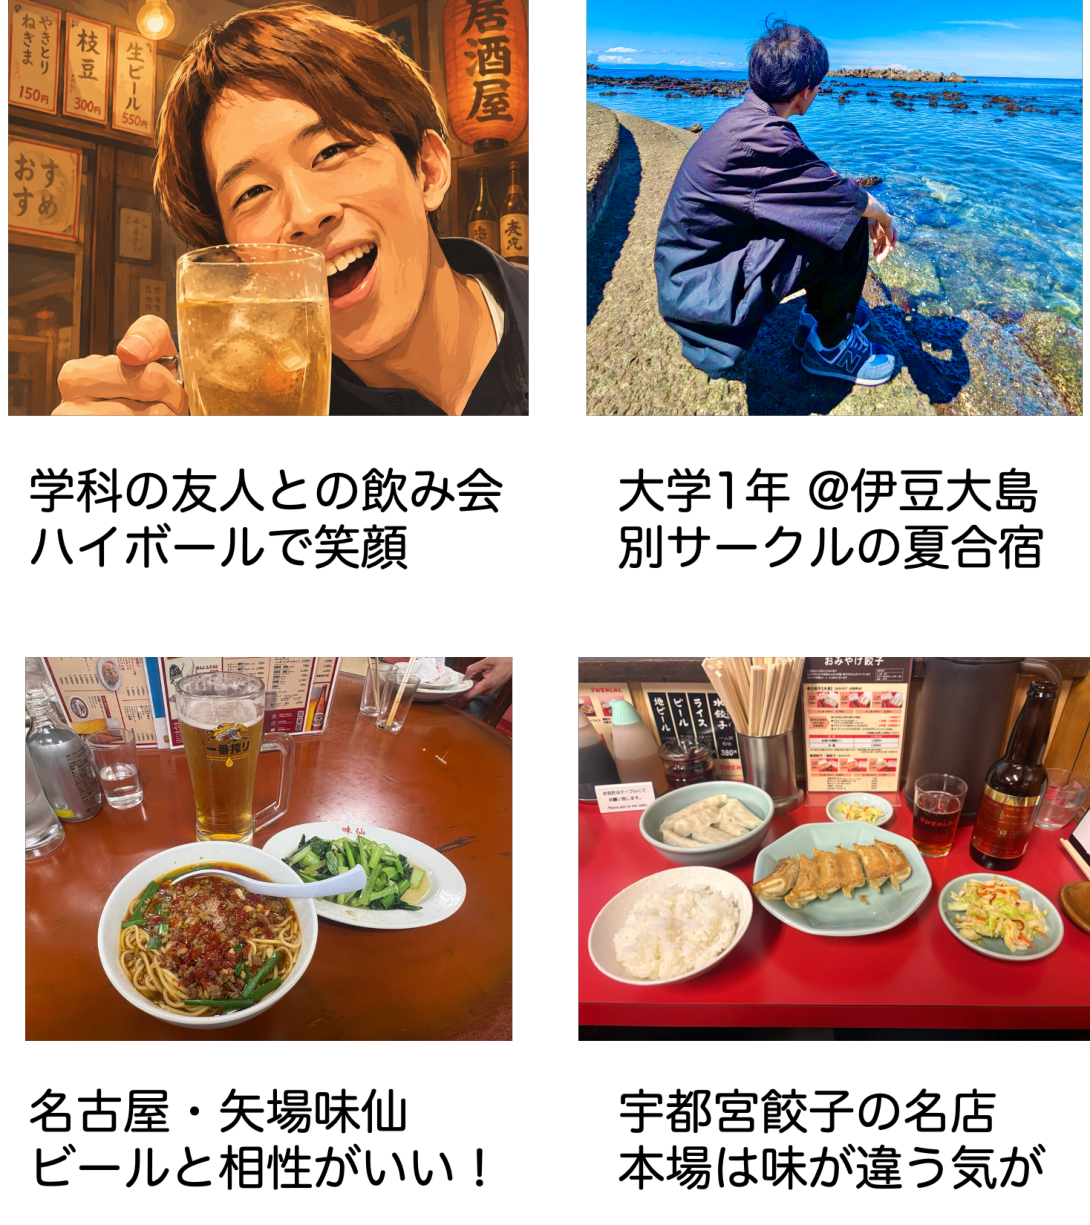
\includegraphics[width=1\textwidth]{self-introduce.pdf} 
        \end{column}
        
        \begin{column}{0.55\textwidth}
          \begingroup
          \footnotesize
          \begin{spacing}{1}
            \begin{itemize}
              \setlength{\itemsep}{0.5pt} 
              \item {\large \textcolor{red!50!blue}{\textsf{INTP 論理学者}}}
              \item 21歳，神奈川県出身，実家暮らし
              \item 横浜国立大理工学部，化学・生命系学科，化学EP
              \begin{itemize}
                \scriptsize
                \item 研究テーマ「自然言語指示に基づく分子生成モデルの開発」
                \item 大学院は内部進学予定です．
              \end{itemize}
              \item 東京大学松尾・岩澤研究室で共同研究インターン
              \item Lumos運営，機械学習PJ主宰者，システムチームメンバー
              \item 以前所属のサークルでケーブルテレビ局の番組制作のリーダーをしていました．
              \item 趣味は様々: 旅行/コーヒー/酒/ゲーム/ラーメン/激辛/ご当地グルメ/名古屋メシ/喫茶店の雰囲気/離島でゆっくり流れる時間を過ごす
            \end{itemize}
          \end{spacing}
          \endgroup
        \end{column}
    \end{columns}
\end{frame}

\section{Transformerとは何か}

\begin{frame}{Transformerとは何か}
  Transformerとは，文章中の単語同士の関係を捉えるための
  ニューラルネットのアーキテクチャである．

  \begin{itemize}
    \item 2017年に翻訳モデルとして提案されるが，画像生成等にも応用されるようになっている．
    \item Attention機構というメカニズムを中心に据える．
    \item 現在のLLMの基盤技術となっている．
  \end{itemize}
\end{frame}

\begin{frame}{Transformerの構造}
  入力
  \begin{itemize}
    \item 文章をトークン列として入力する．
  \end{itemize}
\end{frame}

\section{Attentionの考え方}

\begin{frame}{段組が入るかどうか}
  ちゃんと段組を入れることもできますか？
  
  \begin{columns}
    \centering
    % 左側の列（全体の0.48倍の幅）
    \begin{column}{0.4\textwidth}
      ここに左側の文章や箇条書きを書きます。
      \begin{itemize}
        \item 要素A
        \item 要素B
      \end{itemize}
    \end{column}
    
    % 右側の列（全体の0.48倍の幅）
    \begin{column}{0.4\textwidth}
      ここに右側の画像や文章を書きます。
      %\includegraphics[width=\linewidth]{example-image}
    \end{column}
  \end{columns}
\end{frame}

\begin{frame}{Attentionの考え方}
  以下の\textsf{Example}を理解するとき，どう考えるか？

  \begin{quote}
    私は昨日，\textsf{銀行 bank}に行ってお金を下ろした．
  \end{quote}

  「銀行」を理解するときは，「お金」や「下ろした」との関係に注目します．
\end{frame}

\section{まとめ}

\begin{frame}{まとめ}
  \begin{itemize}
    \item Transformerは単語同士の関係を捉える
    \item Attentionが文脈に応じた重要度を計算する
    \item 現在の大規模言語モデルを支える基盤技術である
  \end{itemize}
\end{frame}

\end{document}